\chapter{Algorithm Design}\label{chapter:algorithmDesign}
\paragraph{}In this section we clarify some fundamental algorithm used by our system in order to achieve its objectives. We will deal basically with high level interactions between the components described in the previous sections.\\
All the algorithms are presented without any reference to a particular programming language but we are assuming an object-oriented paradigm for it.
\paragraph{}Since all the architecture is designed for a client - server interaction an obvious choice of framework would be the \textit{Java Enterprise Edition} framework and so the usage of the Java programming language.

\section{Queue management}
The following algorithm is in charge of the management of the different taxi queues
\begin{algorithm}
\begin{algorithmic}
\REQUIRE $zone:$ a correct taxi zone
\ENSURE a provided taxi or an error message, if there is no taxi driver waiting in the queue \linebreak

\STATE $queues$: map having as keys the taxi zones and as value the corresponding queue \linebreak
$queue:= queues.VALUE(zone)$ \COMMENT {Retrieval of the queue relative to the provided taxi zone} 
$returnValue:$ return value
\IF {$queue.ISEMPTY()$}  
	\STATE{$returnValue:= error$} 
	\ELSE{
		\STATE $taxi:=queue.GETTAXI()$ \COMMENT{Takes the first taxi in the queue}
		\STATE $returnValue:=taxi$
	}
\ENDIF
\RETURN $returnValue$
\end{algorithmic}
\caption{Retrieval of a taxi from a queue}
\end{algorithm}
From the pseudo-code we understand the following:
\begin{itemize}
	\item The QueueManager stores the taxi queues in a map having has key the taxi zones
	\item Each queue is a particular data structure organized with a FIFO policy
\end{itemize}

\begin{algorithm}
\caption{Adding of a taxi to a queue}
\begin{algorithmic}
\REQUIRE{Inputs: \\
	\begin{itemize}
		\item $taxi:$ a taxi driver that must be inserted in a queue
		\item $zone:$ the zone in which the taxi driver wants to operate
	\end{itemize}
}
\ENSURE the adding of the taxi driver to the queue corresponding to the zone provided
\linebreak
\STATE $queues$: map having as keys the taxi zones and as value the corresponding queue \linebreak
$queue:= queues.VALUE(zone)$ \COMMENT {Retrieval of the queue relative to the provided taxi zone} \linebreak
$result = queue.ADDTAXI(taxi)$ \COMMENT{Adding the taxi driver at the bottom of the queue}
\RETURN
\end{algorithmic}
\end{algorithm}
Lets analyze in more detail the data structure $queue$ which has the role of storing the taxi drivers during their waiting of calls: it has a FIFO (\textit{first-in-first-out}) policy for the management of its elements as it is visible in figure \ref{fig:FIFOpolicy}
\begin{figure}[H]
	\centering
	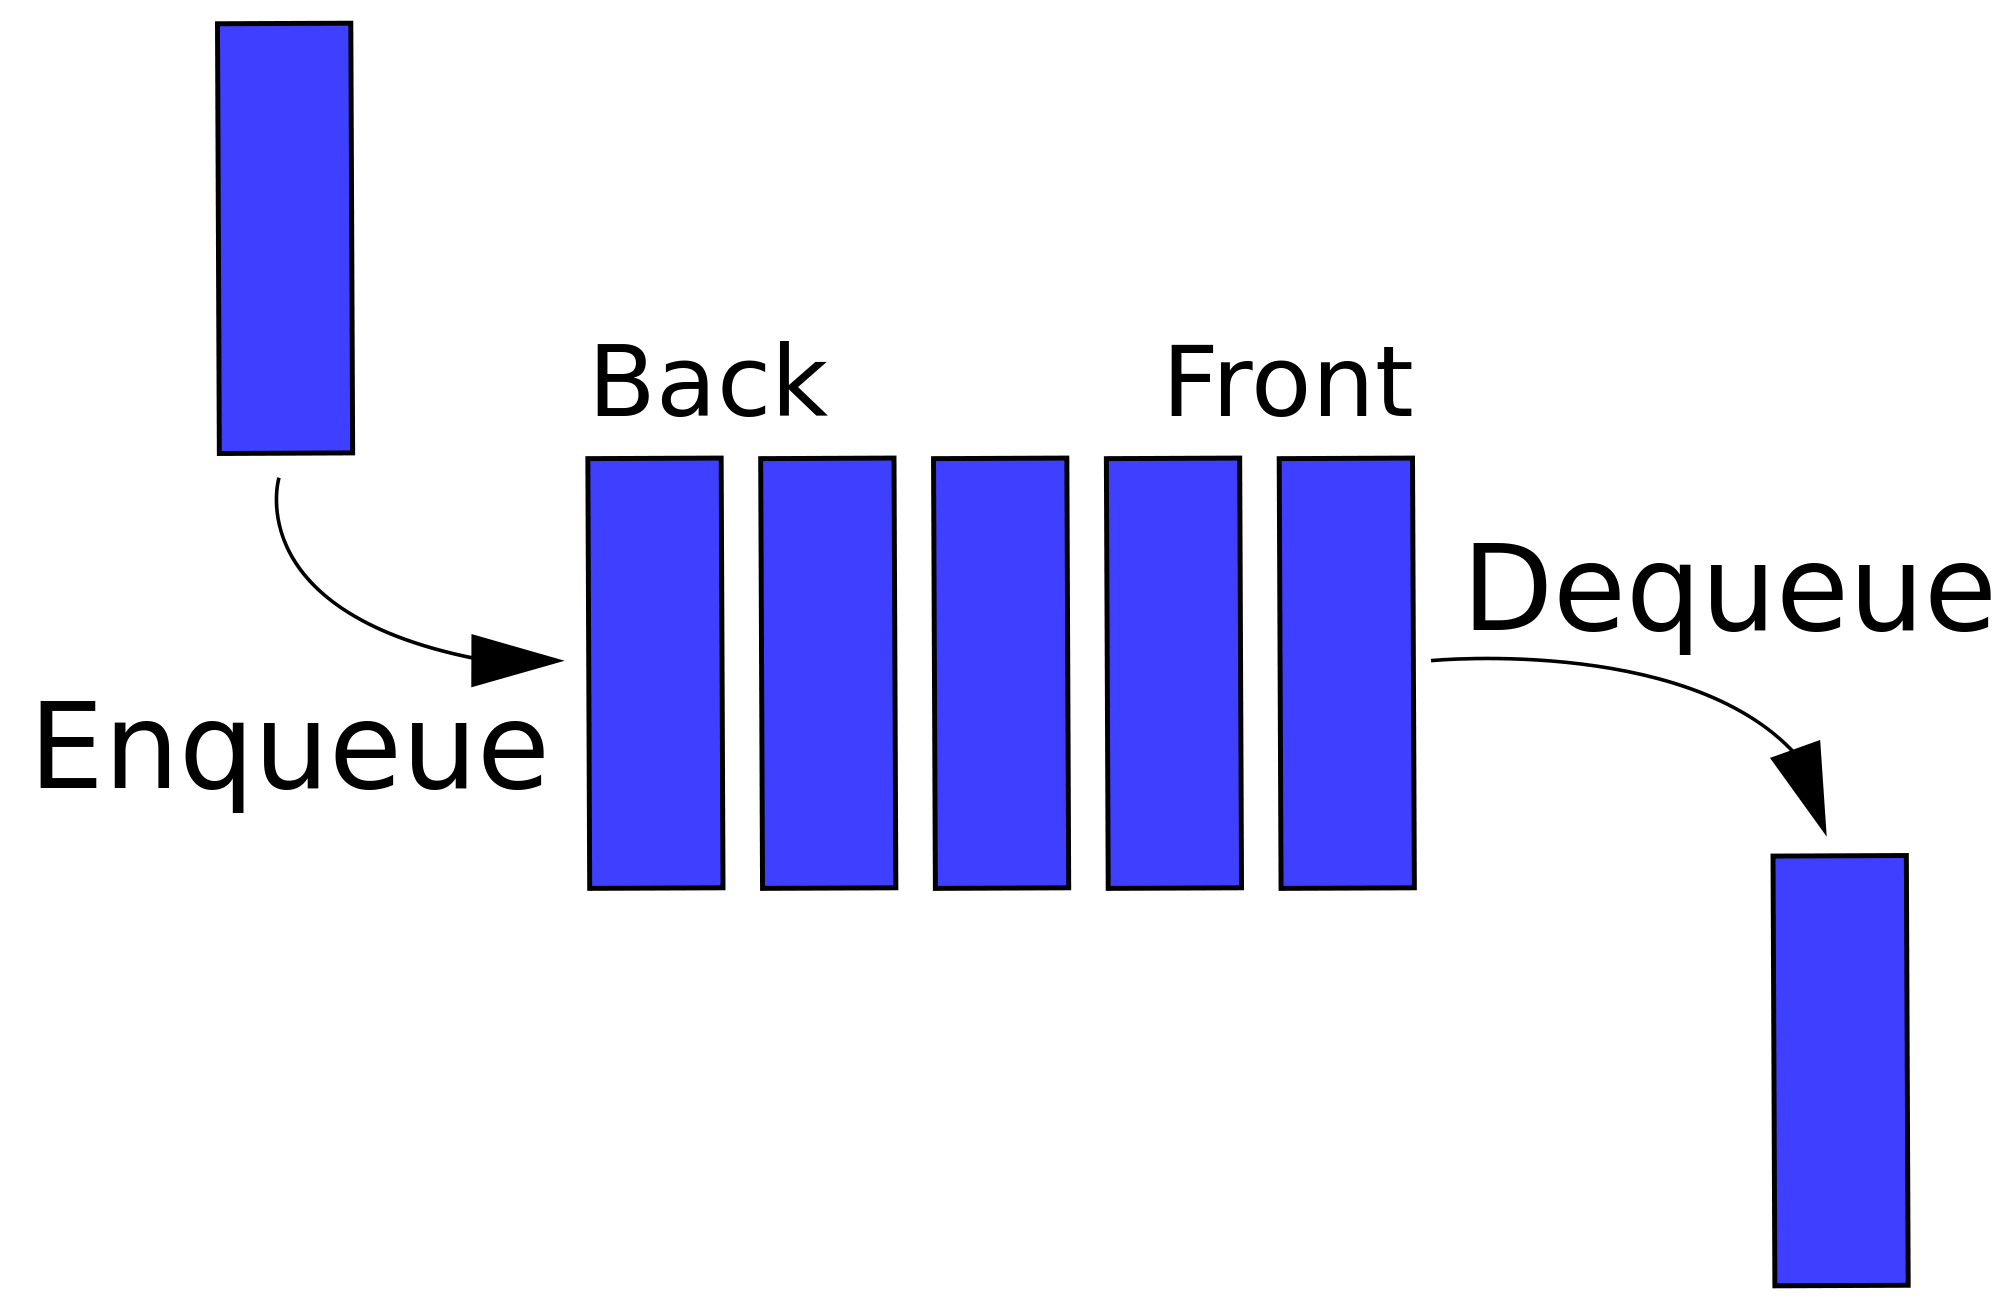
\includegraphics[scale=0.1]{../"Analysis Documents"/FIFO}
	\caption{FIFO policy}
	\label{fig:FIFOpolicy}
\end{figure}
In the Java programming language we could implement a class \texttt{TaxiQueue} which store an element of the class \texttt{Queue}, which is already provided by the framework. Below you can see an example of usage of this class: